\section{GNSS定位基本原理}
\subsection{定位}
\begin{frame}{二维定位模型}
%    \begin{itemize}[<+-| alert@+>] % 当然,除了alert,手动在里面插 \pause 也行
    \begin{itemize}
        \item 信号发射点的位置
        \item 信号接收点与信号发射点的距离
        \item[]
        \begin{figure}
            \centering
            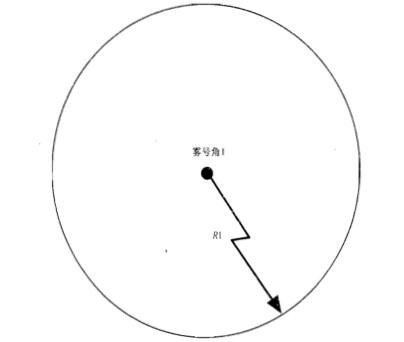
\includegraphics[width=.5\textwidth]{pic/signal_distance.jpg}
            \caption{信号接收点位置分布}
            \label{fig:sig_distance}
        \end{figure}
    \end{itemize}
\end{frame}

\begin{frame}{位置确定}
    \begin{itemize}
        \item \textcolor{red}{三个}信号发射点的位置
        \item 信号接收点与信号发射点的距离
        \item[]
        \begin{figure}
            \centering
            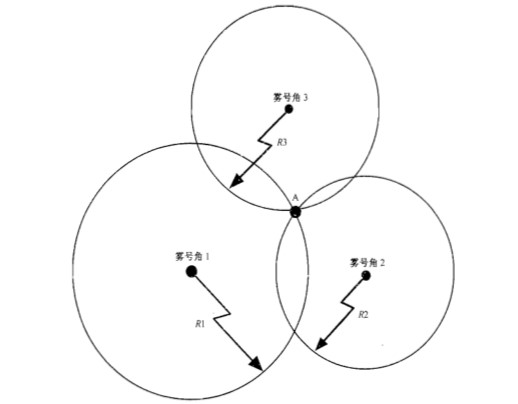
\includegraphics[width=.5\textwidth]{pic/signal_distance_3.jpg}
            \caption{信号接收点位置确定}
            \label{fig:sig_distance_3}
        \end{figure}
    \end{itemize}
\end{frame}

\subsection{坐标系}
\begin{frame}{常用坐标系}
    %\begin{itemize}[<+-| alert@+>]
    \begin{itemize}
        \item 地心地固直角坐标系$\left( \mathrm{ECEF} \right)$
        \begin{itemize}
            \item[] 地心为坐标原点, $OZ$指向北极, $OX$指向参考子午面与地球赤道的交点
        \end{itemize}
        \item 经纬高坐标系$\left( \mathrm{ LLA } \right)$
        \begin{itemize}
            \item[] 地心为坐标原点, 大地高度$h$是过该点到基准椭球面的法线距离
        \end{itemize}
        \item 站心坐标系$\left( \mathrm{ ENU } \right)$
        \begin{itemize}
            \item[] 观测点为坐标原点, 三坐标轴分别指向东, 北, 天方向
        \end{itemize}
    \end{itemize}
\end{frame}

\begin{frame}{坐标变换}
    \begin{itemize}
        \item $\mathrm{LLA} \rightarrow \mathrm{ECEF}$
        \begin{align*}
            x &= \left( N + h \right) \cos \varphi \cos \lambda \\
            y &= \left( N + h \right) \cos \varphi \sin \lambda \\
            z &= \left[ N \left( 1 - \mathrm e ^ 2 \right) + h \right] \sin \varphi
        \end{align*}
        其中,
        \begin{align*}
            \mathrm e &= \sqrt{ 1 - \frac{ b ^ 2 }{ a ^ 2 } } \\
            N &= \frac{ a }{ \sqrt{ 1 - \mathrm e ^ 2 \sin ^ 2 \varphi } }
        \end{align*}
    \end{itemize}
\end{frame}

\begin{frame}{坐标变换}
    \begin{itemize}
        \item $\mathrm{ECEF} \rightarrow \mathrm{LLA}$
        \begin{align*}
            \lambda &= \arctan \frac{ y }{ x } \\
            h &= \frac{ \sqrt{ x ^ 2 + y ^ 2 } }{ \cos \varphi } - N \\
            \varphi &= \arctan \left[ \frac{ z }{ \sqrt{ x ^ 2 + y ^ 2 } }
            \left( 1 - \mathrm e ^ 2 \frac{ N }{ N + h } \right) ^ { -1 }\right]
        \end{align*}
        其中, $h$与$\varphi$组成耦合非线性方程组, 采用迭代方法求解.
    \end{itemize}
\end{frame}

\subsection{卫星星历}
\begin{frame}{星历文件主要参数}
\begin{table}[h!]
    \centering
    \footnotesize
    \caption{星历文件参数}
    \begin{tabular}{ccc}
        \hline
        $t _ { 0e }$ && 星历参考时刻 \\
        $\sqrt{ a }$ && 轨道半长轴的平方根 \\
        $e$ && 轨道离心率 \\
        $i _ 0$ && $t _ { 0e }$时刻轨道倾角 \\
        $\Omega _ 0$ && 升交点经度 \\
        $\omega$ && $t _ { 0e }$时刻近地点幅角 \\
        $M _ 0$ && $t _ { 0e }$时刻平近点角 \\
        $\mathrm d i / \mathrm d t$ && 倾角变化率 \\
        $\mathrm d \Omega / \mathrm d t$ && 升交点经度变化率 \\
        $\Delta n$ && 平均角速度的校正值 \\
        $C _ { uc }$ && 维度幅角余弦修正值 \\
        $C _ { us }$ && 维度幅角正弦修正值 \\
        $C _ { rc }$ && 轨道半径余弦修正值 \\
        $C _ { rs }$ && 轨道半径正弦修正值 \\
        $C _ { ic }$ && 倾角余弦修正值 \\
        $C _ { is }$ && 倾角正弦修正值 \\
        \hline
    \end{tabular}
    \label{tab:ephemeris_para}
\end{table}
\end{frame}

\begin{frame}{计算卫星位置}
    \begin{figure}
        \centering
        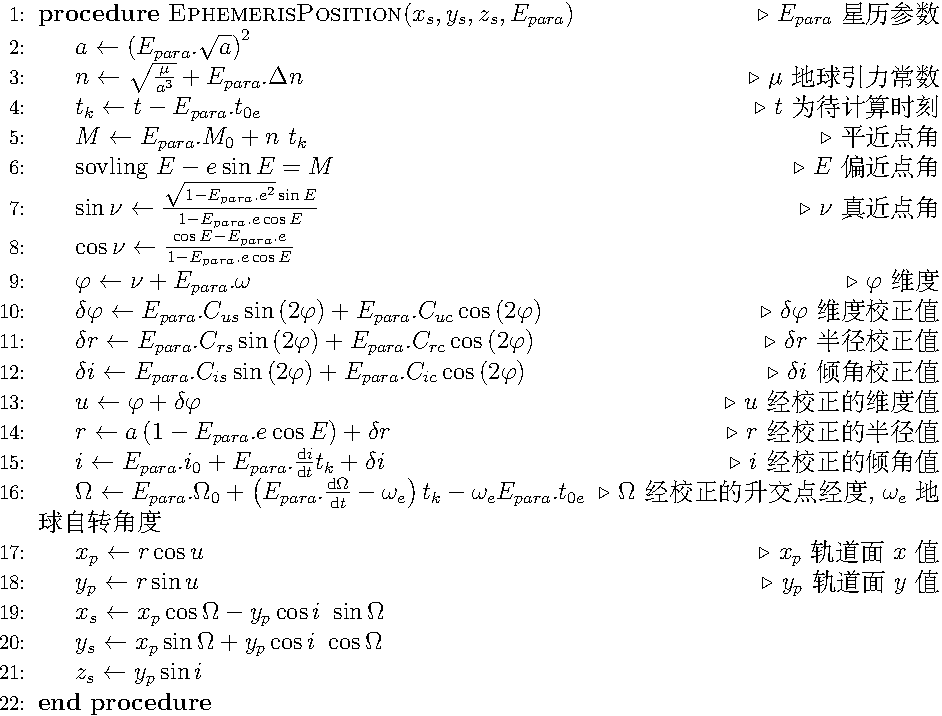
\includegraphics[width = .7\textwidth]{pic/algo_ephemeris.pdf}
        \label{fig:alg_ephemeris}
    \end{figure}
\end{frame}

\subsection{星地距离}
\begin{frame}{记号说明}
    \begin{align*}
        \text{卫星坐标} &: S _ i \left( x ^ { S _ i }, y ^ { S _ i }, z ^ { S _ i } \right), \ i = 1, \ldots, n _ s \\
        \text{接收机坐标} &: R \left( x ^ R, y ^ R, z ^ R \right) \\
        \text{信号离开卫星时刻} &: t _ { S _ i }, \ i = 1, \ldots, n _ s \\
        \text{接收机接收信号时刻} &: t _ R \\
        \text{卫星钟差} &: \delta t _ S \\
        \text{接收机钟差} &: \delta t _ R \\
        \text{接收机载波相位观测值} &: \tilde \varphi _ R ^ { S _ i }, \ i = 1, \ldots, n _ s \\
        \text{光速} &: c
    \end{align*}
\end{frame}

\begin{frame}{测距码}
    \begin{itemize}
        \item R与$S _ i$几何距离$\textcolor{red}{\rho _ R ^ { S _ i }}$
        \begin{align*}
            \textcolor{red}{\rho _ R ^ { S _ i }} &= \sqrt{ \left( x ^ R - x ^ { S _ i } \right) ^ 2
            + \left( y ^ R - y ^ { S _ i } \right) ^ 2
            + \left( z ^ R - z ^ { S _ i } \right) ^ 2 }
        \end{align*}
        \item 信号离开真实时刻$\tau _ { S _ i }$, 接收机接收信号真实时刻$\tau _ R$
        \begin{align*}
            \tau _ { S _ i } &= t _ { S _ i } + \delta t _ S,\
            \tau _ R = t _ R + \delta t _ R
        \end{align*}
        \item 电离层修正值$V _ { \mathrm{ iono, S _ i } } ^ R$, 对流层修正值$V _ { \mathrm{ trop }, S _ i } ^ R$
        \begin{align*}
            \textcolor{red}{\rho _ R ^ { S _ i }} &= c \left( \tau _ R - \tau _ { S _ i } \right)
            + V _ { \mathrm{ iono, S _ i } } ^ R + V _ { \mathrm{ trop }, S _ i } ^ R
        \end{align*}
        \item 伪距${\color{red} \tilde \rho _ R ^ { S _ i } } = c \left( t _ R - t _ { S _ i } \right)$
        \begin{align*}
            {\color{red} \tilde \rho _ R ^ { S _ i } } &= \textcolor{red}{ \rho _ R ^ { S _ i } } - 
            c \textcolor{red}{ \delta t _ R } + c \delta t _ { S _ i }
            - V _ { \mathrm{ iono, S _ i } } ^ R - V _ { \mathrm{ trop }, S _ i } ^ R
        \end{align*}
    \end{itemize}
\end{frame}

\begin{frame}{载波相位}
    \begin{itemize}
        \item 卫星信号载波波长
        \begin{align*}
            \lambda _ 1 &= 19.0 \ \mathrm{ cm },\
            \lambda _ 2 = 24.4 \ \mathrm{ cm }, \
            \lambda _ 3 = 25.5 \ \mathrm{ cm }
        \end{align*}
        \item 接收机收到的载波整周数$\textcolor{red}{N _ R ^ { S _ i }}$
        \begin{align*}
            \textcolor{red}{\tilde \rho _ R ^ { S _ i }} &=
            \lambda \left( \tilde \varphi _ R ^ { S _ i } +
            \textcolor{red}{N _ R ^ { S _ i }} \right) \notag \\
            &= \textcolor{red}{ \rho _ R ^ { S _ i } } - 
            c \textcolor{red}{ \delta t _ R } + c \delta t _ { S _ i }
            - V _ { \mathrm{ iono, S _ i } } ^ R - V _ { \mathrm{ trop }, S _ i } ^ R
        \end{align*}
    \end{itemize}
\end{frame}